\documentclass{article}
\usepackage[utf8]{inputenc}
\usepackage[brazil,english]{babel}
\usepackage[a4paper, total={6in, 8in}]{geometry}
\usepackage{listings}
\usepackage{color}
\usepackage{graphicx}
\usepackage{float}
\usepackage{hyperref}

\definecolor{dkgreen}{rgb}{0,0.6,0}
\definecolor{gray}{rgb}{0.5,0.5,0.5}
\definecolor{mauve}{rgb}{0.58,0,0.82}

\renewcommand{\baselinestretch}{1.5}

\lstset{frame=tb,
  language=Python,
  aboveskip=3mm,
  belowskip=3mm,
  showstringspaces=false,
  columns=flexible,
  basicstyle={\small\ttfamily},
  numbers=none,
  numberstyle=\tiny\color{gray},
  keywordstyle=\color{blue},
  commentstyle=\color{dkgreen},
  stringstyle=\color{mauve},
  breaklines=true,
  breakatwhitespace=true,
  tabsize=3
}

\title{Relatório - Métodos Numéricos (IF816)}
\author{Gabriel Gomes Mendes da Luz\\Universidade Federal de Pernambuco - Centro de Informática}
\date{18 de Outubro de 2018}

\begin{document}
\begin{otherlanguage}{brazil}

\maketitle
\newpage

\tableofcontents

\newpage

\section{Introdução}
    Equações diferenciais ordinárias são equações diferenciais contendo uma ou mais funções de uma variável independente e suas derivadas. O termo \textit{ordinária} indica que ela não deve possuir mais de uma variável independente, como no caso das parciais.\newline
    A importância das EDOs é evidenciada em vários contextos, não só nas áreas científicas, mas também sociais, indo desde a modelagem de fenômenos populacionais, físicos, químicos, até estudos matemáticos, nas áreas de geometria, ou análises de taxas de variação. Assim, seu resultado é muito frequentemente utilizado para fins analíticos, permitindo prever ou simular importantes fenômenos do universo.\newline
    O presente relatório tem, por objetivo, apresentar e discutir sobre os métodos utilizados para solução das EDOs, bem como analisar resultados obtidos durante a execução do projeto da cadeira de Métodos Numéricos para Engenharia da Computação.
\newpage

\section{Métodos}
    Os métodos numéricos são algoritmos utilizados para obter as soluções numéricas das EDOs, através de aproximações, cuja precisão varia de método para método. Basicamente, um método terá seu início em um ponto (ou uma lista de pontos) e irá, em cada passo, usar dos valores anteriores para calcular o valor do próximo ponto no tempo. E assim ele continua, iterativamente, por quanto tempo o for determinado. Existem métodos que são de passos múltiplos ou únicos. O de Euler, como veremos, considera apenas um ponto inicial e vai, passo a passo, andando no tempo, guardando apenas o último valor obtido. Métodos como o de Runge-Kutta tentam aprimorar a precisão dando um "passo intermediário", mas, assim como o de Euler, só retém o valor do último ponto.\newline
    Já os Adams e a Fórmula Inversa, são os chamados métodos de passos múltiplos. Neles, é guardada uma lista com todos os valores previamente calculados. Assim, nesses casos, não usa-se apenas um ponto para o cálculo do próximo, e sim vários anteriores, de acordo com a ordem do método.\newline
    Como esses métodos necessitam de vários valores anteriores, a entrada será, ao invés de um valor $y_0$ e $t_0$, uma lista de valores, de tamanho $ordem - 1$. Ainda, essa lista poderá ser gerada através de outro método, por exemplo, calculando o Adams-Bashforth de ordem 6 a partir de uma lista de 5 valores iniciais gerada pelo método de Runge-Kutta.
    Uma observação importante: todas funções declaradas, a partir do Euler, poderão ser reutilizadas nos métodos seguintes, caso seja necessário, por exemplo, obter uma lista de valores para um método a partir de outro.
    
    \subsection{Métodos por Euler}
        \subsubsection{Euler Simples}
            No método simples, também conhecido como método da reta tangente, as soluções são calculadas de acordo com o tamanho do passo ($h$), quantidade de iterações, a função, ponto ($y_0$) e tempo ($t_0$) iniciais, que são usados na seguinte fórmula:
            \begin{equation}
                y_{n+1} = y_n + h * f(t_n, y_n)
            \end{equation}
            Essa equação é obtida ao nos depararmos com o problema de valor inicial:
            \begin{equation}
                \frac{dy}{dt} = f(t, y)
            \end{equation}
            Onde temos $y(t_0) = y_0$.
            Reescrevendo a equação no ponto $t = t_n$, na forma:
            \begin{equation}
                \frac{d\phi}{dt}(t_n) = f[t_n, \phi(t_n)]
            \end{equation}
            Se aproximarmos essa equação pelo quociente das diferenças correspondente:
            \begin{equation}
                \frac{\phi(t_{n+1}) - \phi(t_n)}{t_{n+1} - t_n} \cong f[t_n, \phi(t_n)]
            \end{equation}
            Substituindo $\phi(t_{n+1})$ e $\phi(t_n)$ pelos seus valores aproximados $y_{n+1}$ e $y_n$, e resolvermos para $y_{n+1}$, iremos obter a fórmula de Euler acima mostrada (1).\newline
            Computacionalmente, a implementação desse método é bastante simples e direta, já este usa apenas o valor atual para calcular o próximo.\newline\newline\newline
 
            \begin{lstlisting}
            def euler_simples(y0, t0, h, qtd_passos, f):
                for i in range(1, qtd_passos + 1):
                    y1 = y0 + f(t0, y0)
                    t1 = t0 + h
                    print('Valor na iteracao %d %lf' % i, y1)
                    y0 = y1
                    t0 = t1
            \end{lstlisting}
        \subsubsection{Euler Inverso}
            Partindo do mesmo princípio que foi usado no Euler Simples, se ao invés dos pontos $y_{n+1}$ e $y_{n}$, forem tomados $y_n$ e $y_{n-1}$, teremos a seguinte equação:\newline
            \begin{equation}
                y_{n} = y_{n-1} + h * f(t_{n}, y_{n})
            \end{equation}
            Adaptando o $n$, ficamos com:
            \begin{equation}
                y_{n+1} = y_n + h * f(t_{n+1}, y_{n+1})
            \end{equation}
            Note que, agora, a equação não é mais explícita: é necessário determinar, de alguma maneira, o valor de $y_{n+1}$ para poder prosseguir com os cálculos. Dessa forma, uma das saídas é usar o método da previsão por Euler Simples: calculamos o ponto $y_{n+1}$ através dele e realizamos a substituição no Euler Inverso. Apesar de não ser o método mais simples do Euler, sua precisão é pior do que a do método simples, além de ter uma implementação ligeiramente mais trabalhada.\newline
            \begin{lstlisting}
            def euler_inverso(y0, t0, h, qtd_passos, f):
                for i in range(1, qtd_passos + 1):
                    y1 = y0 + F(f, t0, y0) # previsao por Euler Simples
                    t1 = t0 + h
                    y1 = y0 + F(f, t1, y1)
                    print('Valor na iteracao %d %lf' % i, y1)
                    y0 = y1
                    t0 = t1
            \end{lstlisting}
        \subsubsection{Euler Aprimorado}
            Agora, numa tentativa de melhoria em relação ao método simples de Euler, ao invés de calcular o ponto usando a função em $(t_n, y_n)$, tomar como resultado o valor nos extremos, consecutivos, ou seja, nos pontos $(t_n, y_n)$ e $(t_{n+1}, y_{n+1})$. Isso seria o equivalente a aproximar a área sobre a curva entre os pontos $t_n$ e $t_{n+1}$. A equação, portanto, será:\newline
            \begin{equation}
                y_{n+1} = y_n + (h / 2) * [f(t_{n+1}, y_{n+1}) + f(t_{n}, y_{n})]
            \end{equation}
            Novamente, apesar da tentativa de aprimoramento, o método ainda conta com um erro de truncamento proporcional a $h^3$. Contudo, em relação a complexidade computacional, o método aprimorado mostra-se mais eficiente: os resultados obtidos por passos de tamanho $h/2$, no método simples, são obtidos neste com passos de tamanho $h$, requerendo, assim, menos iterações. Assim, pode-se obter resultados tão bons quanto no método simples, com um custo computacional significantemente reduzido.\newline
            \begin{lstlisting}
            def euler_aprimorado(y0, t0, h, qtd_passos, f):
                for i in range(1, qtd_passos + 1):
                    y1 = y0 + F(f, t0, y0) # previsao por Euler Simples
                    t1 = t0 + h
                    y1 = y0 + (h / 2) * (F(f, t0, y0) + F(f, t1, y1))
                    print('Valor na iteracao %d %lf' % i, y1)
                    y0 = y1
                    t0 = t1
            \end{lstlisting}
    \subsection{Runge-Kutta (quarta ordem)}
            Neste método, divide-se cada passo em quatro estágios, onde são feitas aproximações do coeficiente angular da reta em três pontos diferentes. Em $k_1$, tem-se o extremo esquerdo, que é o ponto em $t_n$. Em $k_2$, tem-se o ponto médio do passo, entre $t_n$ e $(t_n + h / 2)$. Em $k_3$, é feita uma segunda aproximação do ponto médio. Finalmente, em $k_4$, temos o coeficiente angular no próximo ponto, $(t_n + h)$. Feito isso, o método irá realizar uma média ponderada desses valores parciais obtidos, para chegar em uma "média" do coeficiente angular nesse passo, o que garante uma aproximação muito boa.\newline
            \begin{equation}
                k_1 = f(t_n, y_n)
            \end{equation}
            \begin{equation}
                k_2 = f(t_n + (h / 2), y_n + (h / 2) * k_1)
            \end{equation}
            \begin{equation}
                k_3 = f(t_n + (h / 2), y_n + (h / 2) * k_2)
            \end{equation}
            \begin{equation}
                k_4 = f(t_n + h, y_n + h * k_3)
            \end{equation}
            \begin{equation}
                y_{n+1} = y_n + (h / 6) * (k_1 + 2 * k_2 + 2 * k_3 + k_4)
            \end{equation}
            O método de Runge-Kutta, a depender da implementação e aprimoramentos utilizados, possui, em média, um erro de truncamento local da ordem de $h^5$, o que garante uma precisão duas ordens melhor do que o Euler Aprimorado, e três ordens melhor do que os métodos de Euler Simples e Inverso. Esse método pode ser facilmente implementado, já que é bastante similar ao Euler Simples.\newline
            \begin{lstlisting}
            def runge_kutta(y0, t0, h, qtd_passos, f):
                for i in range(1, qtd_passos + 1):
                    k1 = F(f, t0, y0)
                    k2 = F(f, t0 + h / 2, y0 + (h / 2) * k1)
                    k3 = F(f, t0 + h / 2, y0 + (h / 2) * k2)
                    k4 = F(f, t0 + h, y0 + h * k3)
                    y1 = y0 + (h / 6) * (k1 + 2 * k2 + 2 * k3 + k4)
                    print('Valor na iteracao %d %lf' % i, y1)
                    y0 = y1
                    t0 = t0 + h
            \end{lstlisting}
    \subsection{Métodos dos Adams}
        A partir desta seção, começam os métodos de passos múltiplos. Estes, como foi dito, guardam $N$ valores, onde $N$ é a ordem do método, e usam esses pontos para calcular o próximo. Por conta disso, eles vão apresentar uma precisão consideravelmente melhor do que os métodos lineares das seções $2.1.1$ a $2.2$. Por outro lado, são de implementação mais complexa e, às vezes, necessitam de utilizar a previsão, por outro método, para poder prosseguir no cálculo do próximo ponto (nesses casos, dizemos que o método é \textit{implícito}.\newline
        Um detalhe a ser observado é que, para ordens diferentes, as equações terão coeficientes diferentes. Assim, para que não haja necessidade de copiar as equações, caso a caso, podemos inicializar uma matriz, onde a posição $(i, j)$ contém o $j$-ésimo coeficiente da $i$-ésima ordem do método. Dessa maneira, criamos duas variáveis:
        \begin{description}
          \item[$\bullet$ COEF\_ADAMS\_BASH] - coeficientes para o método de Adam-Bashforth
          \item[$\bullet$ COEF\_ADAM\_MOULTON] - coeficientes para o método de Adam-Moulton
        \end{description}
        Assim, para calcularmos um passo em um desses métodos, podemos criar funções auxiliares f\_bashforth e f\_moulton, que recebem a lista de valores, o tamanho do passo, o tempo inicial e a ordem e retorna o valor do próximo ponto. Para isso, basta seguir a equação do método usado e aplicar os coeficientes de acordo com as matrizes que definimos acima. Na implementação, teremos mais essas duas funções:\newline

        \begin{lstlisting}
            def f_bashforth(funcao, lista_valores, passo_atual, h, t0, ordem):
                y1 = lista_valores[passo_atual - 1]
                k = 0
                for i in range(passo_atual - 1, passo_atual - ordem - 1, -1):
                    yi = lista_valores[i]
                    ti = t0 + i * h
                    fn = F(funcao, ti, yi)
                    y1 += h * fn * COEF_ADAM_BASH[ordem][k]
                    k += 1
                return y1
        \end{lstlisting}
        \begin{lstlisting}
            def f_moulton(funcao, lista_valores, passo_atual, h, t0, ordem):
                y1 = lista_valores[passo_atual - 1]
                k = 0
                for i in range(passo_atual, passo_atual - ordem, -1):
                    yi = lista_valores[i]
                    ti = t0 + i * h
                    fn = F(funcao, ti, yi)
                    y1 += h * fn * COEF_ADAM_MOULTON[ordem][k]
                    k += 1
                return y1
        \end{lstlisting}
        Nos casos em que a lista de valores iniciais deve ser gerada por outro método, ao invés de se ler a lista diretamente da entrada, é passado um ponto inicial $(t_0, y_0)$ para outro método, juntamente ao restante dos parâmetros, e obtê-la. Ao filtrar-se a entrada, isso é feito com uma função que atribui um valor a uma variável e, a partir deste, é possível saber qual a origem dos valores iniciais. No código abaixo, pode-se ver como esse mecanismo é feito, por exemplo, no método de Adam-Moulton:
        \begin{lstlisting}
            if (origem == BY_LISTA_VALORES):
                valores_iniciais = y0
                nome_metodo = 'Adam-Moulton'
            elif (origem == BY_EULER):
                valores_iniciais = euler_simples(y0, t0, h, ordem - 2, funcao, 1)
                nome_metodo = 'Adam-Moulton por Euler Simples'
            elif (origem == BY_EULER_INVERSO):
                valores_iniciais = euler_inverso(y0, t0, h, ordem - 2, funcao, 1)
                nome_metodo = 'Adam-Moulton por Euler Inverso'
            elif (origem == BY_EULER_APRIMORADO):
                valores_iniciais = euler_aprimorado(y0, t0, h, ordem - 2, funcao, 1)
                nome_metodo = 'Adam-Moulton por Euler Aprimorado'
            elif (origem == BY_RUNGE_KUTTA):
                valores_iniciais = runge_kutta(y0, t0, h, ordem - 2, funcao, 1)
                nome_metodo = 'Adam-Moulton por Runge-Kutta'
        \end{lstlisting}
        \subsubsection{Adams-Bashforth}
                Para obter as equações de um método de Adams, a ideia é aproximar $\phi'(t)$ na integral da equação de Euler Simples através de polinômios de ordem igual a quantidade de pontos utilizados na aproximação (mais a frente, será mostrada a integral). Assim, é possível obter uma equação para cada ordem desejada, e quanto maior a ordem, maior a precisão obtida. Para ilustrar, tomemos como exemplo uma aproximação por dois pontos, $(t_n, y_n)$ e $(t_{n-1}, y_{n-1})$, usando um polinômio de grau 1: $P(t) = At + B$. Como o polinômio deve ser uma aproximação, então ele deve satisfazer $P(t_n) = f(t_n, y_n)$. Assim, tem-se que:\newline
                \begin{equation}
                    At_n + B = f_n
                \end{equation}
                \begin{equation}
                    At_{n-1} + B = f_{n-1}
                \end{equation}
                Resolvendo para A e B, conclui-se que:
                \begin{equation}
                    A = \frac{f_n + f_{n-1}}{h}
                \end{equation}
                \begin{equation}
                    B = \frac{f_{n-1}t_{n} - f_{n}t_{n-1}}{h}
                \end{equation}
                A integral na qual realizamos a substituição é:
                \begin{equation}
                    \phi(t_{n+1})-\phi(t_n) = \int_{t_n}^{t_{n+1}} \phi'(t)dt
                \end{equation}
                Substituindo $\phi'(t)$ por $P(t)$ e $\phi(t_{n+1})$ e $\phi(t_n)$ por $y_{n+1}$ e $y_n$, respectivamente, e calculando a integral, chegamos em:
                \begin{equation}
                    y_{n+1} = y_n + h * (\frac{3}{2}f_n - \frac{1}{2} f_{n-1})
                \end{equation}
                Que é a equação para o Adams-Bashforth de ordem 2. No que diz respeito a implementação, supondo recebida a lista de valores iniciais e lembrando também da função auxiliar \textit{f\_bashforth} acima descrita, temos:
                \begin{lstlisting}
                def adams_bashforth(valores_iniciais, t0, h, qtd_passos, funcao, ordem, origem):
                    for passo_atual in range(ordem, qtd_passos + 1):
                        y1 = f_bashforth(f, valores_iniciais, passo_atual, h, t0, ordem)
                        print('Valor no passo %d: %lf' % passo_atual, y1)
                        valores_iniciais.append(y1)
                \end{lstlisting}
                É importante recapitular que o parâmetro "origem" é utilizado no caso em que a lista de valores iniciais provém de outro método, como o Adams-Bashforth recebendo esta do Runge-Kutta, por exemplo.
                Outra observação interessante é que o Adams-Bashforth de grau 0 é, simplesmente, o método de Euler Simples.
                No que diz respeito a precisão, o Adams-Bashforth de segunda ordem possui erro de truncamento local de ordem $h^3$. Contudo, equações mais precisas podem ser obtidas utilizando uma maior quantidade de pontos e gerando polinômios de graus maiores.
        \subsubsection{Adam-Moulton}
            O método de Moulton é uma variação do de Bashforth. Procede-se da mesma maneira, porém, ao invés de utilizarmos os pontos em $t_n$ e $t_{n-1}$, tomam-se $t_n$ e $t_{n+1}$. Aplicando os mesmos cálculos, chegaremos em:
            \begin{equation}
                y_{n+1} = y_n + \frac{1}{2}hf_n + \frac{1}{2}hf_{n+1}
            \end{equation}
            Como pode-se perceber, agora temos uma equação que calcula $y_{n+1}$ de maneira implícita, pois precisamos dos valores para poder substituir em $f_{n+1}$. Assim, faz-se necessário o uso de um método de previsão. Podemos usar o próprio Adams-Bashforth para obter esse valor e, depois, prosseguir com o Moulton. Na implementação, temos:
            \begin{lstlisting}
                def adam_moulton(y0, t0, h, qtd_passos, funcao, ordem, origem):
                    for passo_atual in range(ordem - 1, qtd_passos + 1):
                        y1 = f_bashforth(f, valores_iniciais, passo_atual, h, t0, ordem - 1) #previsao a partir de a. bash.
                        valores_iniciais.append(y1)
                        y1 = f_moulton(f, valores_iniciais, passo_atual, h, t0, ordem)
                        valores_iniciais.pop()
                        print('Valor no passo %d: %lf' % passo_atual, y1)
                        valores_iniciais.append(y1)
            \end{lstlisting}
            Nota-se, também, que o Adam-Moulton de ordem 0 é, simplesmente, o Euler Inverso. O erro de truncamento para o Adam-Moulton de segunda ordem é, de maneira análoga ao Bashforth de mesma ordem, $h^3$.
            Apesar de parecerem métodos bem similares, as fórmulas de Moulton para ordens mais altas possuem uma precisão significantemente melhor do que as de Bashforth, o que é um ponto que o favorece. Porém, por ser implícito, ele possui uma implementação um pouco mais complicada e mais lenta em complexidade assintótica.
    \subsection{Fórmula Inversa de Diferenciação}
        Por fim, para este último método, também surge a necessidade de uma função auxiliar, que calcula o $y_{n+1}$ no $n$-ésimo passo. Da mesma menira que foi feito nos métodos de Bashforth e Moulton, iremos criar uma matriz de coeficientes, dessa vez chamada COEF\_FORM\_INV, e a seguinte rotina:
        \begin{lstlisting}
            def f_inv(funcao, lista_valores, passo_atual, h, t0, ordem):
                t1 = t0 + passo_atual * h
                y1 = lista_valores[passo_atual]
                y1 = COEF_FORM_INV[ordem][0] * h * F(funcao, t1, y1)
                k = 1
                for i in range(passo_atual - 1, passo_atual - ordem - 1, -1):
                    yn = lista_valores[i]
                    y1 += yn * COEF_FORM_INV[ordem][k]
                    k += 1
                return y1
        \end{lstlisting}
        Para obtenção da equação, vamos proceder de forma similar a como foi feito nos Adams. Dessa vez, ao invés de aproximarmos $\phi'(t)$, aproximaremos $\phi(t)$. Assim, iremos diferenciar $P(t)$ e igualar $P'(t_{n+1})$ a $f_{n+1}$, para obtermos uma fórmula implícita para $y_{n+1}$. Daí, usando o mesmo polinômio $P(t) = At + B$, e notando que $P_{1}'(t) = A, P_{1}'(t_{n+1}) = f_{n+1}$, temos:
        \begin{equation}
            At_n + B = y_n
        \end{equation}
        \begin{equation}
            At_{n+1} + B = y_{n+1}
        \end{equation}
            Subtraindo a equação $(19)$ da $(20)$ e substituindo $P'(t)$:
        \begin{equation}
            A = \frac{y_{n-1} - y_n}{h}
        \end{equation}
            Mas, como $A = f_{n+1}$:
        \begin{equation}
            y_{n+1} = y_n + hf_{n+1}
        \end{equation}
            Que é justamente a fórmula do Método de Euler Inverso. O mesmo método pode ser aplicado com mais pontos e polinômios de grau maior, para obter ordens mais altas da Fórmula Inversa.
        \begin{lstlisting}
            def formula_inversa(y0, t0, h, qtd_passos, funcao, ordem, origem):
                for passo_atual in range(ordem - 1, qtd_passos + 1):
                    y1 = f_bashforth(f, valores_iniciais, passo_atual, h, t0, ordem - 1) #previsao a partir de a. bash.
                    valores_iniciais.append(y1)
                    y1 = f_inversa(f, valores_iniciais, passo_atual, h, t0, ordem - 1)
                    valores_iniciais.pop()
                    print('Valor no passo %d: %lf' % passo_atual, y1)
                    valores_iniciais.append(y1)
        \end{lstlisting}
        Por fim, nota-se a que é um método implícito, assim como o Euler Inverso, Aprimorado e Adam-Moulton, e, em vista disso, podemos usar o Bashforth para realizar a previsão.  
\newpage
\section{Resultados}
    Os métodos lineares e mais simples, de passos únicos, possuem uma complexidade melhor do que os métodos de passos múltiplos. Foi realizada uma comparação entre o tempo de execução de cada método, usando a biblioteca timeit de Python, para O PVI $y' = 1 - t + 4y$, com tamanho do passo $h = 0.1$, $y_0 = 0$ e $t_0 = 0$, e sendo executados 20 passos, como veremos na figura 1, nas próximas paginas. Nela, é possível notar que os métodos simples são bem mais rápidos. Porém, essa eficiência pode e geralmente custa na precisão ou na quantidade de passos necessários para atingir certo valor, o que pode terminar deixando o algoritmo lento ou impreciso, que será nossa primeira análise.\newline
    No que diz respeito a precisão dos métodos, ao compará-los com outras soluções, que usam fatores de correção e técnicas mais robustas para aprimoramento dos resultados, foram obtidos valores muito próximos. Nos métodos de passos únicos, os resultados foram praticamente iguais. Porém, nos de passos múltiplos, os resultados foram um pouco distoantes. Uma possível explicação é o fato de utilizar-se poucos pontos anteriores, o que leva o erro de truncamento a ser maior, afinal, usando mais pontos, consegue-se uma precisão melhor. Por isso, para métodos de passos múltiplos, ordens baixas fornecem resultados com precisão fraca, enquanto ordens mais altas conferem uma precisão mais apurada.
    Abaixo, podemos ver uma tabela comparando os resultados obtidos de cada método com a solução exata do PVI $y' = 1 - t + 4y$, $y(0) = 1$, $h = 0.01$, com 200 passos, para a implementação neste relatório especificada:
    

    \begin{table}[!htbp] 
    \centering
     \begin{tabular}{||c c c c c c||}
     \hline
     t & Euler Simples & Euler Inv. & Euler Apr. & Runge-Kutta & Exata \\ [0.5ex] 
     \hline\hline
     0.0 & 1,0000000 & 1,0000000 & 1,0000000 & 1,0000000 & 1,0000000 \\
     0.1 & 1.5952900 & 1.6225210 & 1.6088584 & 1.6090418 & 1,6090418 \\ 
     0.2 & 2.4644587 & 2.5456999 & 2.5047827 & 2.5053298 & 2,5053299 \\
     0.3 & 3.7390345 & 3.9208206 & 3.8289146 & 3.8301387 & 3,8301388 \\
     0.4 & 5.6137119 & 5.9752891 & 5.7917910 & 5.7942258 & 5,7942260 \\
     0.5 & 8.3766864 & 9.0509366 & 8.7074637 & 8.7120037 & 8,7120041 \\
     1.0 & 60.037125 & 70.003323 & 64.830721 & 64.897797 & 64,897803 \\
     1.5 & 426.40817 & 536.94645 & 478.51588 & 479.25913 & 479,25919 \\
     2.0 & 3029.3278 & 4119.6546 & 3532.8788 & 3540.1995 & 3540,2001 \\ [1ex]
     \hline
     \end{tabular}
     \caption{Comparação dos resultados obtidos pelos métodos de passos únicos.}
     \label{table:1}
    \end{table}
    
    \begin{table}[!htbp]
    \centering
     \begin{tabular}{||c c c c c c c||}
     \hline
     t & Lista Inicial & Euler Simples & Euler Inv. & Euler Apr. & Runge-Kutta & Exata \\ [0.5ex] 
     \hline\hline
     0.0 & 1,0000000 & 1,0000000 & 1,0000000 & 1,0000000 & 1,0000000 & 1,0000000 \\
     0.1 & 1.6090418 & 1.6021605 & 1.6157607 & 1.6089502 & 1.6090418 & 1,6090418 \\ 
     0.2 & 2.5053298 & 2.4950453 & 2.5153718 & 2.5051929 & 2.5053298 & 2,5053299 \\
     0.3 & 3.8301388 & 3.8147962 & 3.8451196 & 3.8299346 & 3.8301388 & 3,8301388 \\
     0.4 & 5.7942259 & 5.7713376 & 5.8165747 & 5.7939213 & 5.7942259 & 5,7942260 \\
     0.5 & 8.7120040 & 8.6778586 & 8.7453444 & 8.7115496 & 8.7120040 & 8,7120041 \\
     1.0 & 64.897802 & 64.645500 & 65.144156 & 64.894444 & 64.897802 & 64,897803 \\
     1.5 & 479.25918 & 477.39490 & 481.07951 & 479.23437 & 479.25918 & 479,25919 \\
     2.0 & 3540.2000 & 3526.4248 & 3553.6505 & 3540.0167 & 3540.2000 & 3540,2001 \\ [1ex]
     \hline
     \end{tabular}
     \caption{Comparação dos resultados obtidos pelo método de Adams-Bashforth, onde o nome da coluna representa o método que gerou a lista de valores iniciais.}
     \label{table:2}
    \end{table}
    
    \begin{table}[!htbp] 
    \centering
     \begin{tabular}{||c c c c c c c||} 
     \hline
     t & Lista Inicial & Euler Simples & Euler Inv. & Euler Apr. & Runge-Kutta & Exata \\ [0.5ex] 
     \hline\hline
     0.0 & 1,0000000 & 1,0000000 & 1,0000000 & 1,0000000 & 1,0000000 & 1,0000000 \\
     0.1 & 1.6090418 & 1.6035236 & 1.6144257 & 1.6089684 & 1.6090418 & 1,6090418 \\ 
     0.2 & 2.5053298 & 2.4970977 & 2.5133616 & 2.5052203 & 2.5053298 & 2,5053299 \\
     0.3 & 3.8301388 & 3.8178579 & 3.8421209 & 3.8299754 & 3.8301388 & 3,8301388 \\
     0.4 & 5.7942259 & 5.7759051 & 5.8121011 & 5.7939822 & 5.7942259 & 5,7942260 \\
     0.5 & 8.7120040 & 8.6846725 & 8.7386707 & 8.7116404 & 8.7120040 & 8,7120041 \\
     1.0 & 64.897802 & 64.695848 & 65.094844 & 64.895116 & 64.897802 & 64,897803 \\
     1.5 & 479.25918 & 477.76693 & 480.71514 & 479.23933 & 479.25918 & 479,25919 \\
     2.0 & 3540.2000 & 3529.1737 & 3550.9581 & 3540.0534 & 3540.2001 & 3540,2001 \\ [1ex]
     \hline
     \end{tabular}
     \caption{Comparação dos resultados obtidos pelo método de Adam-Moulton, onde o nome da coluna representa o método que gerou a lista de valores iniciais. Obs: previsão por Adams-Bashforth.}
     \label{table:3}
    \end{table}
    
    \newpage
    
    \begin{table}[!htbp] 
    \centering
     \begin{tabular}{||c c c c c c c||}
     \hline
     t & Lista Inicial & Euler Simples & Euler Inv. & Euler Apr. & Runge-Kutta & Exata \\ [0.5ex] 
     \hline\hline
     0.0 & 1,0000000 & 1,0000000 & 1,0000000 & 1,0000000 & 1,0000000 & 1,0000000 \\
     0.1 & 1.6090418 & 1.6028277 & 1.6151070 & 1.6089591 & 1.6090418 & 1,6090418 \\ 
     0.2 & 2.5053298 & 2.4961154 & 2.5143233 & 2.5052072 & 2.5053298 & 2,5053299 \\
     0.3 & 3.8301388 & 3.8163943 & 3.8435538 & 3.8299560 & 3.8301388 & 3,8301388 \\
     0.4 & 5.7942260 & 5.7737217 & 5.8142387 & 5.7939532 & 5.7942260 & 5,7942260 \\
     0.5 & 8.7120043 & 8.6814154 & 8.7418597 & 8.7115973 & 8.7120043 & 8,7120041 \\
     1.0 & 64.897806 & 64.671783 & 65.118409 & 64.894799 & 64.897806 & 64,897803 \\
     1.5 & 479.25922 & 477.58913 & 480.88927 & 479.23700 & 479.25922 & 479,25919 \\
     2.0 & 3540.2004 & 3527.8600 & 3552.2450 & 3540.0362 & 3540.2004 & 3540,2001 \\ [1ex]
     \hline
     \end{tabular}
     \caption{Comparação dos resultados obtidos pelo método da Fórmula Inversa de Diferenciação, onde o nome da coluna representa o método que gerou a lista de valores iniciais. Obs: previsão por Adams-Bashforth.}
     \label{table:4}
    \end{table}
    
    Como foi possível ver nos resultados obtidos, dentre os métodos de passo único, o Runge-Kutta e Euler Aprimorado é o que apresenta maior proximidade à solução exata, enquanto o Euler Simples e Inverso se distanciam bastante, o que confirma o erro de truncamento de cada um ($h^5, h^3, h^2$ e $h^2$, respectivamente). Já nos métodos de passos múltiplos, vemos resultados muito mais precisos do que os de passos únicos, chegando bem próximos à solução exata. Na especificação do projeto, foram dadas entradas com um passo muito grande ($h = 0.1$), poucas iterações e ordens baixas, o que causava, muitas vezes, uma discrepância nos resultados, uma vez que a precisão dos métodos de passos múltiplos está diretamente atrelada ao grau do polinômio e, principalmente, ao tamanho do passo. É como se quiséssemos aproximar uma curva através de retas: quanto menor cada reta, mais fiel seremos à curva original. Assim, se quisermos uma precisão muito boa, o ideal seria combinar passos muito pequenos a um método de ordem alta. Contudo, como podemos ver abaixo, na figura 1, a complexidade fica maior: tamanha precisão é custosa para métodos mais complexos (passos múltiplos). A figura apresenta o tempo de execução estimado de cada método, para o PVI $y' = 1 - t + 4y$, $y(0) = 0$, $h = 0.1$, com 20 passos. 

    \begin{figure}[!htbp] 
      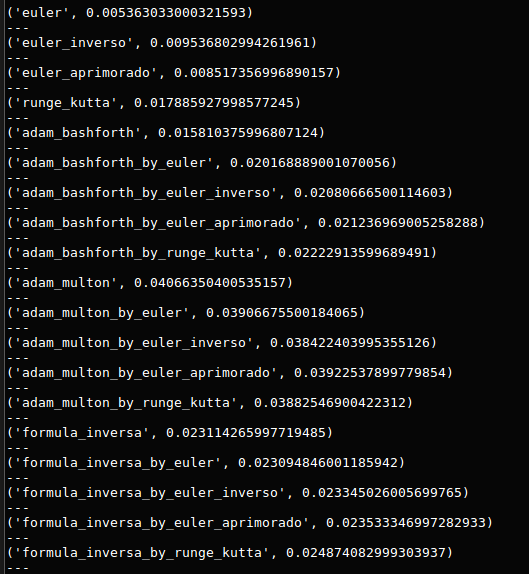
\includegraphics[width=\linewidth]{pic1.png}
      \caption{Comparação de tempos de execução dos métodos. (nome do método a esquerda, tempo de execução (segundos) a direita)}
      \label{fig:pic1}
    \end{figure}
\newpage
\section{Referências Bibliográficas}
        \begin{description}
          \item[$\bullet$] {Boyce, William E., 1930 - Equações diferenciais elementares e problemas de valores de contorno / William E. Boyce,
Richard C. DiPrima tradução e revisão Valéria de Magalhães Iório. - Rio de Janeiro :
LTC, 2010.}
          \item[$\bullet$] {Linear Multistep Method. Wikipedia. Disponível em:  \url{https://en.wikipedia.org/wiki/Linear\_multistep\_method}. Acesso em 17 out. 2018.}
          \item[$\bullet$] {SymPy 1.3 Documentation. Sympy. Disponível em: \url{https://docs.sympy.org/latest/index.html}. Acesso em 17. out. 2018.}
          \item[$\bullet$] {Pyplot tutorial - Matplotlib 2.0.2 documentation. Matplotlib. Disponível em: \url{https://matplotlib.org/users/pyplot_tutorial.html}. Acesso em 17. out. 2018.}
        \end{description}
\end{otherlanguage}
\end{document}
